\begin{figure}[H]
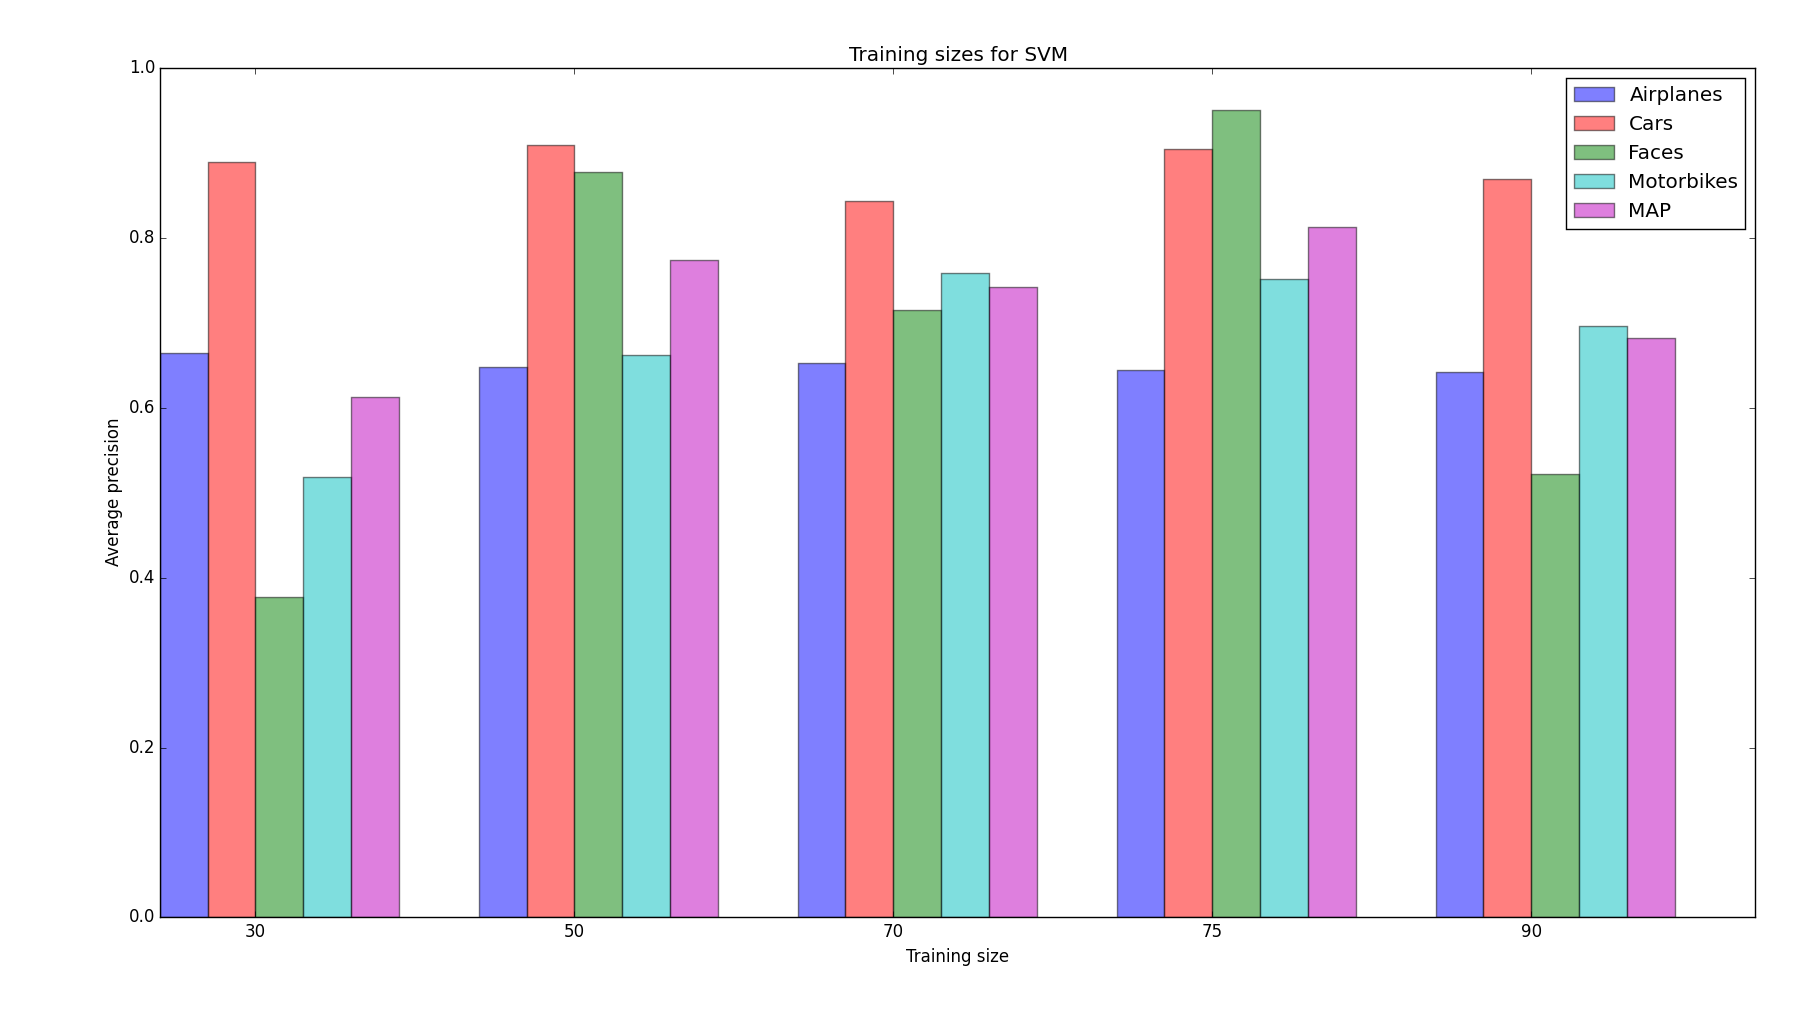
\includegraphics[width=\textwidth]{../plots/training_size_SVM}
\caption{Effect of training size for SVMs on AP}
\end{figure}

\begin{table}[H]
\begin{tabular}{|c|ccccc|}
\hline
\textbf{Training samples} & \textbf{AP Airplanes} & \textbf{AP Cars} & \textbf{AP Faces} & \textbf{AP Motorbikes} & \textbf{MAP}\\
\hline
30 & 0.6647 & 0.8898 & 0.3772 & 0.5184& 0.6125\\
50 & 0.6484 & 0.9096 & 0.8780 & 0.6627 & 0.7747\\
70 & 0.6531 & 0.8441 & 0.7156 & 0.7590 & 0.7429\\
75 & 0.6447 & 0.9053 & 0.9510 & 0.7516 & 0.8132\\
90 & 0.6426 & 0.8697 & 0.5227 & 0.6963 & 0.6828\\
\hline
\end{tabular}
\caption{Effect number of training samples (per class) for SVM, Sift type: dense, Color space: opponent}
\end{table}
